% Files using this must be two subfolders
% deep. Adjust the number of ../ for the
% depth of the file.
% Imports
\usepackage{fancyhdr}
\usepackage{geometry}
\usepackage{icomma}
\usepackage{amsmath}
\usepackage{multicol}
\usepackage{mathptmx}
\usepackage{anyfontsize}
\usepackage{t1enc}
\usepackage{tabto}
\usepackage{listings}
\usepackage{filecontents}
\usepackage{subcaption}
\usepackage{tikz}
\usepackage[parfill]{parskip}
\usepackage{graphicx}
\usepackage[]{mdframed}
\usepackage{amsmath}
\usepackage[makeroom]{cancel}
\usepackage{pgfplots}
\usepackage{pgfplotstable}
\usepackage{xfrac}
\usepackage{amssymb}
\usepackage{mathtools}
\pgfplotsset{compat=1.18}
\usetikzlibrary{patterns}
\usepgfplotslibrary{polar}
\usepgfplotslibrary{fillbetween}

\geometry{margin=2.5cm}

\newcommand{\name}{Kaleb Burris}
\newcommand{\classname}{MATH F253, Elizabeth S. Allman, University of Alaska Fairbanks}
\newcommand{\assignment}{FILL IN ASSIGNMENT NAME}

\pagestyle{fancy}

\fancyhead[L]{
    \name 
    \newline
    \classname
    \newline
    \assignment
}

\newcommand{\horizontal}{\noindent\rule{\hsize}{0.4pt}}

\setlength{\headheight}{42pt}
\setlength{\headsep}{0.25in}
\setlength{\columnsep}{0.35cm}
\setlength{\columnseprule}{1pt}

\usepackage[T1]{fontenc}
\usepackage{lmodern}

\usepackage{enumitem}
\usepackage{graphicx}
\graphicspath{ {./lab07images/} }

% Put class number, class name, and professor 
% name.
% Use only in case of emergency, this
% should be covered by the preamble.
% \renewcommand\classname{}

% Put the assignment name with \S if 
% necessary for the section and the question 
% numbers.
\renewcommand\assignment{Lab 7: The Ballistic Pendulum and Projectile Motion, 3/20/2023, Partners: Maite Valentin-Lugo, Seth Waln}

\begin{document}

    % Templates
    \iffalse
    % Use these for equations.
    \begin{equation*}
        \begin{gathered}
            Equations go here.
        \end{gathered}
    \end{equation*}

    % Use this if a line of math is too long.
    \resizebox{\hsize}{!}{$Long equation goes here$}

    % Use these for multiple columns.
    \begin{multicol*}{# of columns}
        % Remove the * if you want the columns to be balanced.
    \end{multicol*}

    % Use this to add a horizontal line.
    \horizontal

    \fi

    % Begin homework here.
    %%%%%%%%%%%%%%%%%%%%%%

    \begin{enumerate}
        \item [1.]
        \begin{align*}
            p_{i}   & = m \cdot v_{ix}      \\
            p_{f}   & = (M+m) \cdot v_{fx}  \\
            v_{ix}  & = \frac{p_{f}}{m}     \\
                    & = \boxed{\frac{(M+m) \cdot v_{fx}}{m}}
        \end{align*}

        \item [2.]
        \begin{align*}
            E_{i}   & = \frac{1}{2}(M+m)(v_{fx})^{2}    \\ 
        \end{align*}

        \item [3.]
        \begin{align*}
            E_{f}   & = \frac{1}{2}(M+m)(g)(\Delta h)   \\
            E_{i}   & = E_{f}                           \\
            V_{ix}  & = \sqrt{2g\Delta h}               \\
            v_{ix}  & = \frac{(M+m) \cdot v_{fx}}{m}    
                      = \boxed{\frac{(M+m)\sqrt{2g\Delta h}}{m}}
        \end{align*}

        \item [4.]
        \begin{align*}
            y - y_{0}   & = y_{1}                       \\
            y_{l}       & = \frac{1}{2}gt^{2}           \\
            t           & = \boxed{\sqrt{\frac{2y_{1}}{g}}}
        \end{align*}

        \item [5.]
        \begin{align*}
            \Delta x    & = v_{ix} \cdot t                  \\
            \Delta x    & = \frac{(M+m)\sqrt{2g\Delta h}}{m} \cdot 
                            \boxed{\sqrt{\frac{2y_{1}}{g}}} \\
        \end{align*}

        \item [6.]
        \begin{align*}
            m   & = 0.0661 \pm 0.00005 kg                   \\
            M   & = 0.1648 \pm 0.00005 kg                   \\  
        \end{align*}

        \pagebreak

        \item [7., 8., 9.]
        
        \resizebox{\hsize}{!}{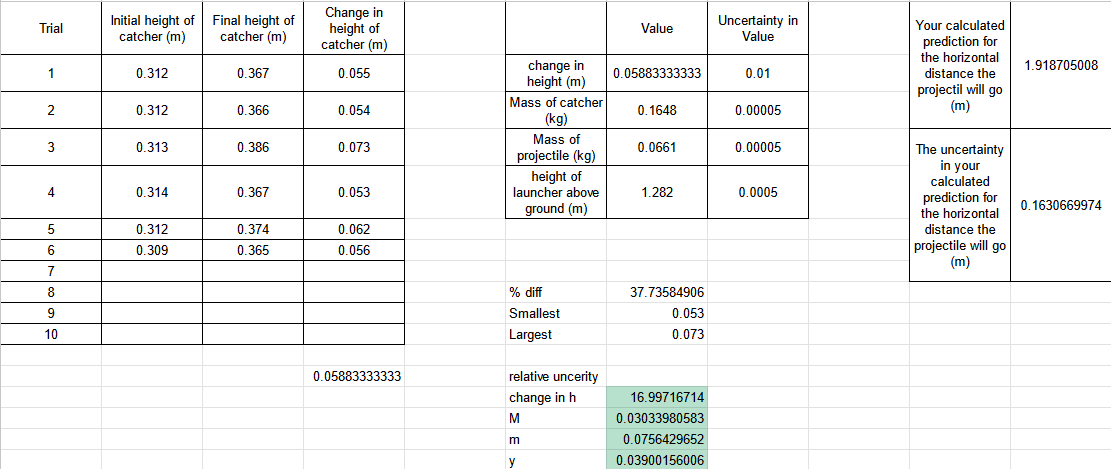
\includegraphics{image-01}}
        
        \item [10.]
        
        \begin{align*}
            \Delta x    & \stackrel{\text{Excel}}{=} 1.9187 m
        \end{align*}

        \item [11.]
        
        \begin{gather*}
            \delta x = \sqrt{
                \left(\frac{2}{0.0661}\sqrt{1.9187 \cdot 1.282}(0.00005)\right)^{2} +
                \left(\frac{-2(0.1648)}{0.0661^{2}}\sqrt{1.9187 \cdot 1.282}(0.00005)\right)^{2} +
                \left(\left(1+\frac{0.1648}{0.0661}\right)\sqrt{\frac{1.282}{0.5883}(0.00005)}\right)^{2} +
                \left(\left(1+\frac{0.1648}{0.0661}\sqrt{\frac{1.282}{0.5883}}(0.00005)\right)\right)^{2}
            }
            = \boxed{\pm 0.1631 m}
        \end{gather*}

        \item [12.]
        
        The force of gravity only determines how far the projectile travels in the y-axis, not the x-axis, and so, although it determines long the projectile is in the air, it does not affect how far it's traveling.
        
        \item [13.]
        
        \begin{equation*}
            1 - (0.73 / 0.53) \approx 0.3775
        \end{equation*}

        The percent difference between the largest and smallest $\Delta h$ was $\approx$ 37.75\%. This is acceptable because our largest value was an extreme outlier. All other data points were within $\pm 0.1$ m of each other.

        \item [14.]
        
        The change in height uncertainty was the heighest, which makes sense given how our units of measurement were less precise and many more forces were acting against the accuracy of the height compared to the others.

        \item [15.]
        
        Once we were able to establish the correct angle to fire at, we struck the target almost perfectly.

        \item [16.]
        
        The theoretical and experimental values were extremely similar, with some loss in the experimental values.

        \item [17.]
        
        If we overshot, our $\Delta h$ would have been too high, as having a larger starting height ($\Delta h$) results in more time for the projectile to move, and thus more distance for it to travel through.

        \item [18.]
        
        We did not account for air resistance or friction between the ball and the gun, although because of the aerodynamic nature of the projectile and the fact that the measurements are done after the ball leaves the gun, those two forces, especially in a toy case such as this, are extremely negligible, as was shown when we tried the experiment. The main change I would make is to have an clearer instructions as we spent most of our time initially trying to figure out what exactly ``Attach a thread to the catcher and string it through the Velcro on the upper base of the launcher'' meant, along with an error later on related to $y_{l}$ and $\Delta y$.

    \end{enumerate}

\end{document}